\documentclass{article} % For LaTeX2e
\usepackage{nips13submit_e,times}
\usepackage{hyperref}
\usepackage{epsfig}
%\usepackage{mahnig}
\usepackage{url}
\usepackage{enumerate}
\usepackage{booktabs}
\usepackage{graphicx}
\usepackage{float}

%\documentstyle[nips13submit_09,times,art10]{article} % For LaTeX 2.09




\title{URL Categorization}


\author{Domantas Meidus}

% The \author macro works with any number of authors. There are two commands
% used to separate the names and addresses of multiple authors: \And and \AND.
%
% Using \And between authors leaves it to \LaTeX{} to determine where to break
% the lines. Using \AND forces a linebreak at that point. So, if \LaTeX{}
% puts 3 of 4 authors names on the first line, and the last on the second
% line, try using \AND instead of \And before the third author name.

\newcommand{\fix}{\marginpar{FIX}}
\newcommand{\new}{\marginpar{NEW}}

\nipsfinalcopy % Uncomment for camera-ready version

\begin{document}


\maketitle



\begin{abstract}
  In this document we report our proposal for the application of supervised classification methods to the URL Categorization problem. The classifiers that we have selected for the classification tasks were: Logistic regression, Decision Trees, KNeighbors. I have implemented the classification process using the scikit-learn, nltk, numpy, urlib, BeautifulSoup and langdetect libraries. The classifiers is learnt by using the train data and computing the accuracy in the test data. From our results the best accuracy has been produced by the Logistic Regression Classifier.
\end{abstract}

\section{Description of the problem}
 
 The task we have to solve is the classification of the  ``URL categorization'', introduced in the project task. 
 
 The dataset includes category which each URL belongs to. The goal of the project is to predict the category of URL, among as many categories.

  The database has the following characteristics: 

\begin{itemize}
  \item $18$ attributes.
  \item $25$ categories:
  	\subitem 1 News\_and\_Media
  	\subitem 2 Career\_and\_Education
  	\subitem 3 Internet\_and\_Telecom
  	\subitem 4 Sports
  	\subitem 5 Games
  	\subitem 6 Books\_and\_Literature
  	\subitem 7 Law\_and\_Government
  	\subitem 8 Travel
  	\subitem 9 Finance
  	\subitem 10 Arts\_and\_Entertainment
  	\subitem 11 Reference
  	\subitem 12 Autos\_and\_Vehicles
  	\subitem 13 Adult
  	\subitem 14 Business\_and\_Industry
  	\subitem 15 People\_and\_Society
  	\subitem 16 Shopping
  	\subitem 17 Health
  	\subitem 18 Pets\_and\_Animals
  	\subitem 19 Home\_and\_Garden
  	\subitem 20 Beauty\_and\_Fitness
  	\subitem 21 Gambling
  	\subitem 22 Recreation\_and\_Hobbies
  	\subitem 23 Science
  	\subitem 24 Computer\_and\_Electronics
  	\subitem 25 Food\_and\_Drink
\end{itemize}


\section{Description of our approach}
  
 The implementation of the project according to the tasks:

\begin{enumerate} 

 \item Design any preprocessing of the web pages in the dataset.

 \item Define and learn the classifier using the training data.

 \item  Design the validation method to evaluate the accuracy of the proposed classification approach.
 
\end{enumerate} 


\subsection{Preprocessing}

 For preprocessing data these steps have been made:
 
 \begin{enumerate}
 	
	 	\item Using urlopen \cite{url_open} html content of URL is downloaded and with BeautifulSoup tool it is converted to the plain text if URL ''Main category'' is not 'Not working' and main\_category:confidence value is greater than 0.5.
 	\item Using langdetect tool by plain URL text program detect language which is used in URL content.
 	\item If detected language is english and URL domain belongs to 'com', 'org', 'net', '.us', '.uk', '.au' or '.ca' domains - text is tokenize by using nltk tool. 
 	
 	These actions is done for all URL from URL categorization file.
 	
 	\item After all URL is filtered, our program determinate which categories are compatible with cross validation predict method: if each category is used more than the number of cross validation predict parameter CV, that means that category can be predicted by cross validation predict method. Take note that Cross validation accepts those classes which have minimum 2 of training data.
 	
 	These applicable categories are marked as classifier \b{labels}.
 	
 	\item For each category top 50 words which are the most frequently used in URL is stored in list excluding ''stop words'' and symbols in range 32-64 and 91 - 96 decimal values which represented in ASCII table (\href{http://www.asciitable.com/}{http://www.asciitable.com/}).
 	
 	\item Vector with zero values is created for each URL with top 50 words for each category. If each filtered URL top most frequently words contains categories used most frequently words, then value of word position in vector is changed to value 1.
 	
 	After this action vector representation of each filtered URL is marked as classifier \b{features}.
 	
 \end{enumerate} 
	
  The data was split into two different sets: train and test, for validation. We use the same train set to learn all the classifiers, and the same test set for evaluating their accuracy.


\subsection{Classifiers}

 We use three different classifiers:

  \begin{enumerate}   
    \item Logistic regression
    \begin{itemize}
    	\item C=1.0
    	\item class\_weight=None 
    	\item dual=False
    	\item fit\_intercept=True 
    	\item intercept\_scaling=1
    	\item max\_iter=100 
    	\item multi\_class='ovr'
    	\item n\_jobs=1 
    	\item penalty='l2'
    	\item solver='liblinear'
    	\item tol=0.0001
    	\item verbose=0
    	\item warm\_start=False 
    \end{itemize}
    \item Decision trees
    \begin{itemize}
    	\item class\_weight=None 
    	\item criterion='gini'
    	\item max\_depth=None 
    	\item max\_features=None
    	\item max\_leaf\_nodes=None
    	\item min\_impurity\_decrease=0.0'
    	\item min\_impurity\_split=None 
    	\item min\_samples\_leaf=1
    	\item min\_samples\_split=2
    	\item min\_weight\_fraction\_leaf=0.0
    	\item presort=False
    	\item random\_state=None
    	\item splitter='best'
    \end{itemize}
  	\item KNeighbors with parameters:
      \begin{itemize}
      	\item algorithm='auto' 
      	\item leaf\_size=30
      	\item metric='euclidean'
      	\item metric\_params=None
      	\item n\_jobs=1
      	\item n\_neighbors=5
      	\item p=2
      	\item weights='uniform'
      \end{itemize}
   \end{enumerate}

For each classifier, these were the parameters by default of the scikit-learn library. 
 
\subsection{Validation}
 
 To validate our results we compute the classifier accuracy in the test data. Another possibility was to compute the cross-validation in the complete dataset but we used the split between train and test because it was simpler. 

 As an additional validation step we computed the confusion matrices for the twenty four classifiers.
 
\section{Implementation}
 All the project steps were implemented in Python. Libraries that was used in the project: urlib and BeautifulSoup for downloading URL and parsing HTML code into plain text, langdetect for language detection from plain text, numpy for using data structures to store labels and features information and scikit-learn for the classification tasks. Illustration how the implementation works in the Python notebook \texttt{URL-categorization-Jupyter-Notebook.ipynb}.


\section{Results}
The highest score performance comparing of all 3 classifiers has Logistic Regression. The score results are displayed in table~\ref{tab:lr_score}.
The score results for each class displayed for Logistic Regression ~\ref{fig:lr_scores.png} figure, Decision tree ~\ref{fig:dc_score.png} figure, KNeighbors ~\ref{fig:kn_score.png} figure.
\begin{table}[H]
	\centering
	\begin{tabular}{lrrrr}
		 &   \textbf{Logistic Regression}     &  \textbf{Decision tree}     &  \textbf{KNeighbors} \\\hline
		\toprule \hline
		Precision score:     &  0.40 &   0.28 &   0.23 \\\hline
		recall:     &   0.49 &   0.28 &   0.11 \\\hline
		f1-score:     &   0.46 &   0.28 &   0.09 \\\hline
		Accuracy score:     &   0.49 &   0.28 &   0.10 \\\hline
		\bottomrule \hline
	\end{tabular}
	\caption{Scores produced by Logistic Regression.}
	\label{tab:lr_score}
\end{table}	

\begin{figure}[H]
	\minipage{0.32\textwidth}
	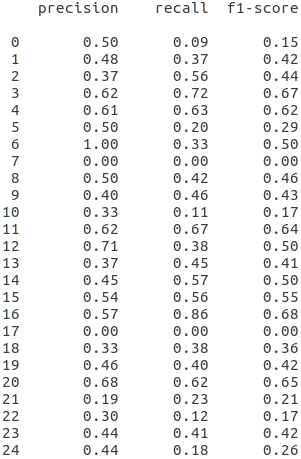
\includegraphics[width=\linewidth]{lr_scores.png}
	\caption{Logistic Regression scores for each class}\label{fig:lr_scores.png}
	\endminipage\hfill\hfill\hfill\hfill\hfill\hfill
	\minipage{0.32\textwidth}
	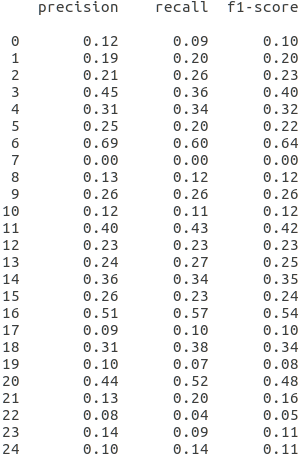
\includegraphics[width=\linewidth]{dc_score.png}
	\caption{Decision Tree scores for each class}\label{fig:dc_score.png}
	\endminipage\hfill\hfill\hfill\hfill\hfill\hfill
	\minipage{0.32\textwidth}%
	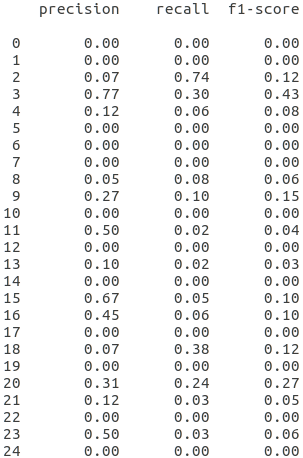
\includegraphics[width=\linewidth]{kn_score.png}
	\caption{KNeighbors scores for each class}\label{fig:kn_score.png}
	\endminipage
\end{figure}

 
 The results of the computation of the confusion matrices for  Logistic regression, Decision tree and KNeighbors classifiers are respectively shown in Tables~\ref{fig:lr_con.png}, \ref{fig:dc_con.png} and~\ref{fig:kn_con.png}.
\hfill
\begin{figure}[H]
	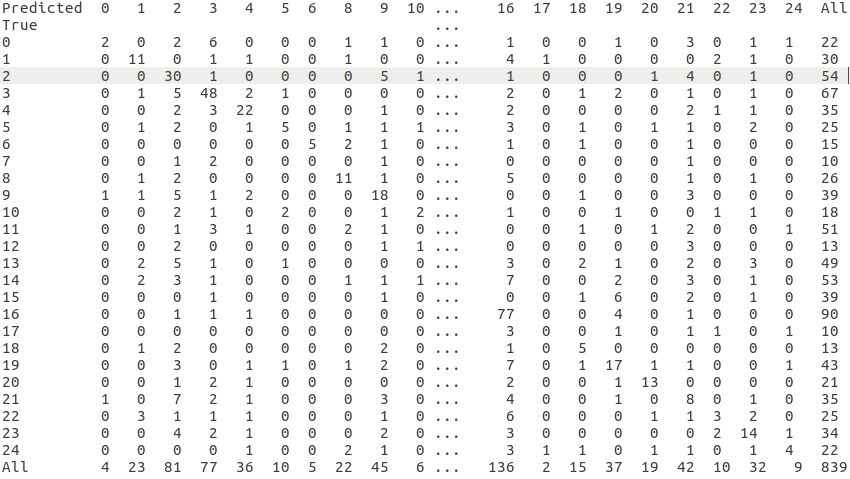
\includegraphics[width=\linewidth]{lr_con.png}
	\caption{Logistic Regression confusion matrix}
	\label{fig:lr_con.png}
\end{figure}
\hfill
\begin{figure}[H]
	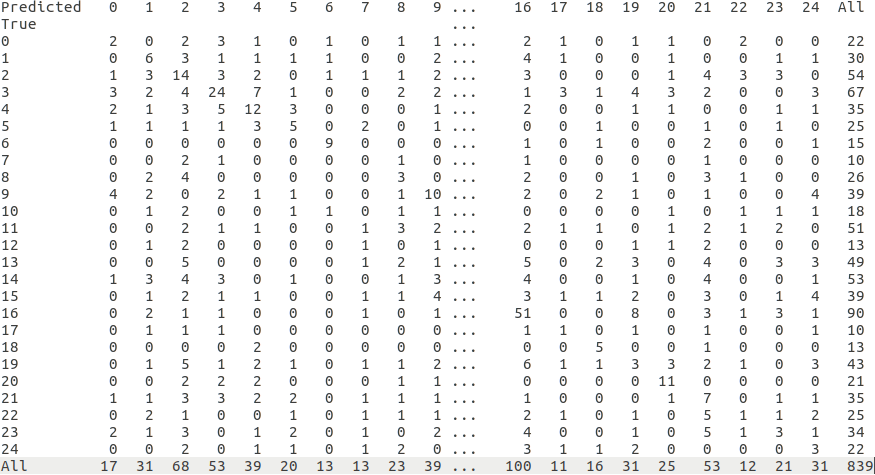
\includegraphics[width=\linewidth]{dc_con.png}
	\caption{Decision tree confusion matrix}
	\label{fig:dc_con.png}
\end{figure}
\hfill
\begin{figure}[H]
	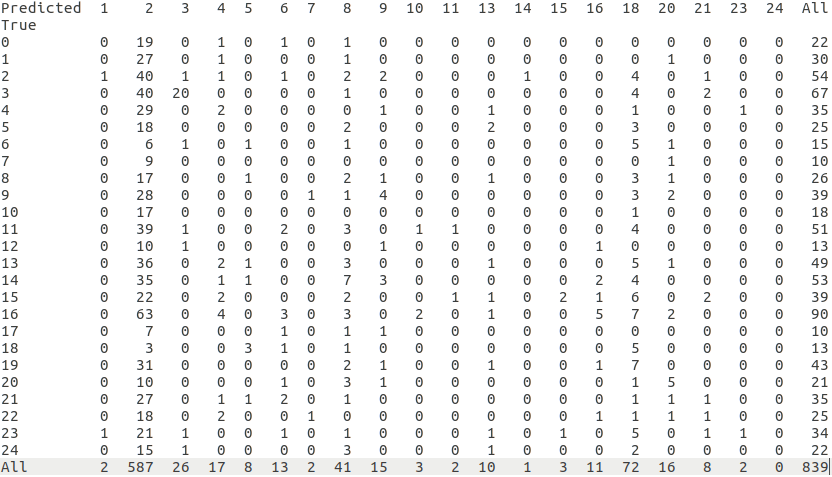
\includegraphics[width=\linewidth]{kn_con.png}
	\caption{KNeighbors confusion matrix}
	\label{fig:kn_con.png}
\end{figure}

\section{Conclusions}
  In our project we have applied  Logistic regression, Decision tree and KNeighbors classifiers  to the ``URL categorization'', introduced in \cite{url_class}. We have computed the accuracy of these classifiers and observed that:
  \textbf{Logistic regression} produces the highest accuracy. We have also observed, from the analysis of the confusion matrices, that Logistic Regression produced poor discrimination between the People\_and\_Society and an Health categories. Also, it was poorly trained to detect Pets\_and\_Animals category.\\
  \textbf{KNeighbors} was poorly trained to detect Pets\_and\_Animals category.\\
  \textbf{Logistic regression} produced poor discrimination between the Health and an Internet\_and\_Telecom. Also, for this classifier it was unable to define Food\_and\_Drink category.
	
  
 \bibliographystyle{unsrt}
 \bibliography{bibtex_references_project}

\end{document}
